\documentclass[hyperref={pdfpagelabels=false}]{beamer}
\let\Tiny=\tiny
\mode<presentation>{
\usetheme{Singapore}
%\usecolortheme{lily}
\usefonttheme{serif}
}
\usepackage{default}
%\usepackage{ucs}
\usepackage[utf8]{inputenc}
\usepackage{gb4e}
\usepackage[T1]{fontenc}
\usepackage{ tipa }
\usepackage{qtree}
\usepackage{synttree}
\usepackage{color}
\usepackage{tree-dvips}
\usepackage[absolute,overlay]{textpos}
%\usepackage{covington-beamer}
\usepackage{lmodern}
\usepackage{natbib}
\usepackage{graphicx}

%\usepackage{memoir}
%\usepackage{relsize}
%\newcommand{\subscript}[1]{\raisebox{-0.25em}{\smaller #1}}
%\logo{\includegraphics[height=0.5cm]{hilogo2.png}}
\setbeamertemplate{footline}[frame number] 
%gets rid of navigation symbols
\setbeamertemplate{navigation symbols}{}

\title{One Very Slow Change: the decline of relative clause extraposition}
\author{Joel C. Wallenberg\\Newcastle University\\
    \texttt{joel.wallenberg@ncl.ac.uk}}
\institute{Bad Data Workshop}
%\date[]{March 18, 2013 \\ University of Oslo}

\begin{document}

\begin{frame}[plain]
\titlepage
\end{frame}

\begin{frame}
\frametitle{Some Challenges for Dealing with Bad (diachronic) Data}
\begin{itemize}
	\item Resolution of our observations
	\item Time-depth
	\item Sources of noise
	\item Cross-linguistic comparison
	\item Acquisition's link to diachronic patterns of incrementation, diffusion, etc.
%	\item \textbf{In the tradition of \citep{wlh1968}, our hypotheses about the problems of language change are becoming sufficiently precise (at a mathematical level) that they are increasingly difficult to test with the data at hand, even as data becomes better.}
\end{itemize}
\end{frame}

\begin{frame}
\frametitle{Some Challenges for Bad Data}
\begin{itemize}
	\item \textbf{Our hypotheses about the problems of language change are becoming sufficiently precise that they are increasingly difficult to test with the data at hand, even as data becomes better.}
	\item \nocite{wlh1968} Weinreich, Labov, \& Herzog (1968) identified, among others, the following problems for a theory of language change, which are also questions about acquisition:
	\begin{itemize}
		\item \textbf{actuation} of new variants.
		\item \textbf{constraints} on possible changes (and possible stability).
		\item \textbf{transition} between language states (maybe reducible to the others?).
		\item \textbf{embedding} of the change in larger linguistic and extralinguistic systems.
	\end{itemize}
\end{itemize}
\end{frame}

\begin{frame}
\frametitle{Production data for linguistic research\\(e.g. parsed corpora)}
\begin{itemize}
%	\item If we want to use data from language use, possibly language use over time, then we need the following;
	\item \textbf{Linking Hypotheses for linguistic structure:} link linguistic theory to the quantitative patterns of language use, by finding clear quantitative predictions of hypotheses about linguistic structure.
	\item \textbf{Statistical Reasoning:} in probabilistic (stochastic) data, find the patterns underlying the noise (without accidentally modeling the noise).
	\item Example of a successful linking hypothesis is the ``Constant Rate Hypothesis'' \citep[][and many subsequent]{kroch1989}:
		\begin{itemize}
			\item If one syntactic parameter has a number of different surface realizations, and that parameter changes over time, then changes in the different surface contexts will occur at the same rate.
		\end{itemize}

\end{itemize}
\end{frame}

\begin{frame}
\frametitle{Production data for linguistic research}
\begin{center}
	\textbf{Linking Hypotheses for acquisition:} link our theory of acquisition to the quantitative patterns of language use, by finding clear quantitative predictions of specific hypotheses about the acquisition process.
\end{center}
\end{frame}



\begin{frame}
\frametitle{Outline}
\tableofcontents
\end{frame}

\section{Imperfect Specialization}
%Finnish example? tough movement example?
%do verb particles, do sound change example and stable variation example (optionality)

\subsection{The diachronic blocking effect and the Principle of Contrast}

\begin{frame}{Introduction}
	Variation in grammar is often described as falling into one of two categories.
	
	\begin{enumerate}
		\item Competing Grammars
		\begin{itemize}
			\item Leads to language change via the \textbf{replacement} of one grammatical object by another.
%			\item Competition is parameterized in some fashion, as in competing flavors of the same functional head \citep{kroch1994}.
		\end{itemize}
		\item Optionality (within a grammar?)
		\begin{itemize}
			\item Diachronically stable variation between grammatical processes.
		\end{itemize}
	\end{enumerate}
	
\end{frame}


\begin{frame}{Introduction}
	\textbf{Overall Hypothesis:} all variation, including grammatical optionality, is formally \textbf{competing grammars}, with the following consequences (\citealt{fruehwaldwallenberg2013}, \textsl{In Prep}): \nocite{fruehwaldwallenberginprep}
	\begin{itemize}
		\item We expect variation (apparent optionality) between two grammatical forms to be diachronically unstable.
		\item True(st) optionality = stable(st) variation, and its difference from usual language change must be explained by some aspect of language use outside of the linguistic variable itself (\textbf{embedding}), which slows the change. 
%		\item The linguistic system (and therefore the variation) interacts with various dimensions of language use, which have their own characteristics. 
%the (in)stability of a competing grammars situation
		\item We argue that it depends on the mathematical character of some dimension (i.e. external to the variable's grammar) with which the variation interacts (\textbf{embedding}).
			\begin{itemize} \item Partial specialization of categorical variants along a continuous dimension. \end{itemize}
%		\item Optionality in grammar must also be parameterized. The implications of this point are greater for stable phonological variation.
	\end{itemize}

\end{frame}

\begin{frame}
\frametitle{Blocking and Contrast}
\begin{block}{``Blocking Effect'' \citep{aronoff1976}}
	\begin{itemize}
		\item General pressure against two forms existing for one function (``doublet''), unstable \citep{kroch1994}.
		\item[ ]\{\textsl{lough, laughed}\} (laugh-\textsc{pst}; ME, \citealt{taylor1994}) \\ \{\textsl{jimmies, sprinkles}\} (candy topping, Philadelphia)\\ \{\textsl{melted, molten}\}
		%\item The possible historical outcomes of a doublet are replacement (one form left) or specialization (forms diverge in function).
	\end{itemize}
\end{block}
\begin{block}{``Principle of Contrast''}
	\begin{itemize}
		\item A strategy that children use in acquiring language: assume that two forms have two meanings (or uses)\citep[][{ \it inter alia}]{clark1987, clark1990}.
		\item Children hypothesize that novel words also refer to novel objects \citep[as in][among many other replications of the effect]{markmanwachtel1988}.
	\end{itemize}
\end{block}
%\begin{itemize}
%	\item General cognitive pressure against two forms existing for one function (``doublet''). 
%	\item This is the ``blocking effect'', as described for morphosyntactic doublets in Kroch (1994).\nocite{kroch1994}
%	\item The possible historical outcomes of a doublet are replacement (one form left) or specialization (forms diverge in function).
%	\item Crucially, they do not coexist forever, nor does one variant die randomly.
%	\item Part of the blocking effect is a language acquisition strategy, the ``Principle of Contrast'' (E. Clark 1987); \citep[cf. also][and references therein]{clark1990}. \nocite{clark1987}
%\end{itemize}
\end{frame}


\begin{frame}
\frametitle{Blocking = Contrast + Evolutionary Dynamics}
\begin{itemize}
	\item A doublet is two variants competing for finite resources, as in e.g. biological evolution.
		\begin{itemize} 
			\item Instead of competing for something like food, they are competing for use (time in the mouths/brains of speakers). 
	%		\item \textbf{Selection} operates on the number of times a variant is heard (and accurately analyzed) by an acquirer.
			\end{itemize}
	\item Either one variant has an advantage, and so \textbf{replaces} the other \citep[often following a logistic function;][]{nowak2006}.
	\item Or neither variant has an advantage (or much of one), in which case random walk and drift (which can also lead to \textbf{replacement}).
	\item But in linguistic doublets, there is always the counter-pressure to resolve the doublet through \textbf{specialization}, because of the Principle of Contrast.
\end{itemize}
\end{frame}




\begin{frame}
\frametitle{Doublets = Competing Grammars \citep{kroch1994}}
\begin{itemize}
	\item[ ] \textbf{``Competing Grammars'', general form}: 2 variants are available to a speaker, in the relevant inventory of grammatical formatives, with overlapping functions (e.g. the same meaning).
		\begin{itemize}
			\item E.g. two featural versions of the same syntactic head. 
			\item E.g. two different output mappings for the same phonological input.
			\item E.g. two different Spell-outs of a morpheme.
			\item E.g. two different adjunction sites.
		\end{itemize}
	\item[ ] A fact about language use: at some point in the derivation, the speaker reaches a \textbf{decision-point}.
		\begin{itemize}
		\item The speaker has a choice between formatives to continue the derivation, and either will result in a grammatical utterance, and a meaning close enough to the speaker's intention (the resulting meanings overlap).
		\item It is speaker ``choice'' more in the sense of an urn problem.
		\end{itemize}
		%SAY: the decision point exists because the different formatives exist, and that is competing grammars. Note that if they don't overlap in meaning, then the situation still exists formally, but there is no real decision 
		%Say something about adjunction
\end{itemize}
\end{frame}



\begin{frame}
\frametitle{Doublets = Competing Grammars}
\begin{itemize}
	\item Necessary for the description of \textbf{any} linguistic change in a categorical dimension.
		\begin{itemize} 
			\item E.g. word-order parameters \citep{pintzuk1991, santorini1992}; a phonological rule like German final stop devoicing (Fruehwald, Gress-Wright, \& Wallenberg 2009)\nocite{fruehwaldgresswallenberg2013}. 
			\item In any such case, a speaker in the middle of the change in progress (code-)switches between categorical variants \citep{kroch1989}.
		\end{itemize} 
\end{itemize}
\end{frame}


\begin{frame}
\frametitle{Summary: Blocking and Contrast}
So, doublets are Competing Grammars, and Contrast plus evolutionary dynamics yield the outcomes \textbf{replacement} and \textbf{specialization}.\\
\vspace*{10mm}
Whether replacement occurs depends on whether specialization can arrest it.

\end{frame}


\begin{frame}
\frametitle{Consequence: Blocking and Contrast}
\begin{itemize}
	\item If specialization occurs, its effect depends on the \textbf{domain of specialization}. A change can be:
		\begin{enumerate}
			\item A replacement change in progress (outright competition going to completion).
			\item A specialization change in progress (specialization for different functions going to completion).
			\item \textbf{``Stable'' variation, or optionality:} variants have \textbf{imperfectly specialized} along a continuous (or ordinal) dimension, e.g. style, prosodic weight. 
		\end{enumerate}
	\item If categorical variants specialize along a categorical dimension, complete specialization should eventually result.
	\item If categorical variants specialize along a continuous or ordinal dimension, then complete specialization can \textbf{never} result, but replacement can be slowed by \textbf{imperfect specialization}.
\end{itemize}

\end{frame}



\section{Very Slow Change}
\subsection{The Loss of Relative Clause Extraposition}

\begin{frame}{A Very Slow Change}
\begin{itemize}
    \item One consequence of our overall hypothesis is that some things that didn't look like change turn out to be.
    \item Relative clause extraposition is a change in progress, but a very slow one \small{\citep[][]{wallenbergunderrev, wallenberg2013b, fruehwaldwallenberginprep}}.
        \begin{itemize}
        \item It has been mischaracterized as syntactic optionality.
        \end{itemize}
    \item The study used the same coding query (with minor adaptation) on 7 parsed diachronic corpora (4 language histories).
    \item Both the time-depth and cross-linguistic dimensions were necessary in order to discover the change.
    \item Only because we had both dimensions were we able to observe (and confirm) the slowest syntactic change discovered to date.
    \end{itemize}
\end{frame}

\begin{frame}{Case Study: Relative Clause Extraposition}

	\begin{block}{French}
		\begin{exe}
			\ex \gll mais l'heure vient $[$que je ne parleray plus a vous en proverbes$]$\\
			but {the time} comes { }that I \sc{neg} speak-\sc{fut} more to you in proverbs\\
			\quad ``The time approaches when I will no longer speak to you in parables''\\
			(MCVF, 1523-NEW-TESTAMENT-P, A5V.2491)
		\end{exe}
	\end{block}
	
	\begin{block}{English}
		\begin{exe}
			\ex All had now been tried $[$which either threats or promises, forbearance or
fatherly chastisement, could effect$]$.\\
			(PPCMBE, FROUDE-1830,2,2.20; date: 1830)
		\end{exe}
	\end{block}

%\begin{block}{Icelandic}
%		\begin{exe}
%			\ex \gll stjarna væri sén í landnorðri frá Jemen, er Kómeta heitir\\
%			1861.ORRUSTA.NAR-FIC,.784)
%		\end{exe}
%	\end{block}

\end{frame}



\begin{frame}{Hypotheses for the diachronic study}
\begin{itemize}
    \item \textbf{Hypothesis 1:} Relative clause position (a binary variable) is specialized along a continuous dimension, weight, and so it should be \textbf{nearly} stable, but not entirely stable.
%            \begin{itemize}
   %     \item \textbf{Theory:} all variation is really change, competition between variants \small{\citep{kroch1989}}, of some kind.
   %     \end{itemize}
    \item \textbf{Hypothesis 2:} All IE relative clauses derive historically from clause-adjoined relatives \small{\citep{kiparsky1995}}.
        \item \textbf{Hypothesis/Suggestion 2':} The old clause-adjoined kind are still around, in the form of extraposition, and the change Kiparsky proposed hasn't finished yet \small{\citep{wallenbergunderrev}}.
    \end{itemize}

\end{frame}



\subsection{Specialization for weight}

\begin{frame}{Specialization within individuals}
\begin{itemize}
	\item Relative clause extraposition in the Parsed Corpus of Early English Correspondence  (PCEEC; \citealt{pceec}).
	\item Allows us to look at reasonable samples from individual speakers (letter-writers), as well as an historical sample from 1400--1700.
	\item Coded for prosodic weight of the relative clause, in number of words, from 0--50.
%	\item Also coded for extraposition from Subject vs. Object.
\end{itemize}
	\textbf{Hypothesis:} individual speakers treat weight as a continuous variable, with extraposition specialized imperfectly along it \citep[as suggested by][]{antonmackenzie2011a}.

\end{frame}


%Splice in two plots of speakers


\begin{frame}{All PCEEC, over time (N = 8073 clauses)}

\begin{center}
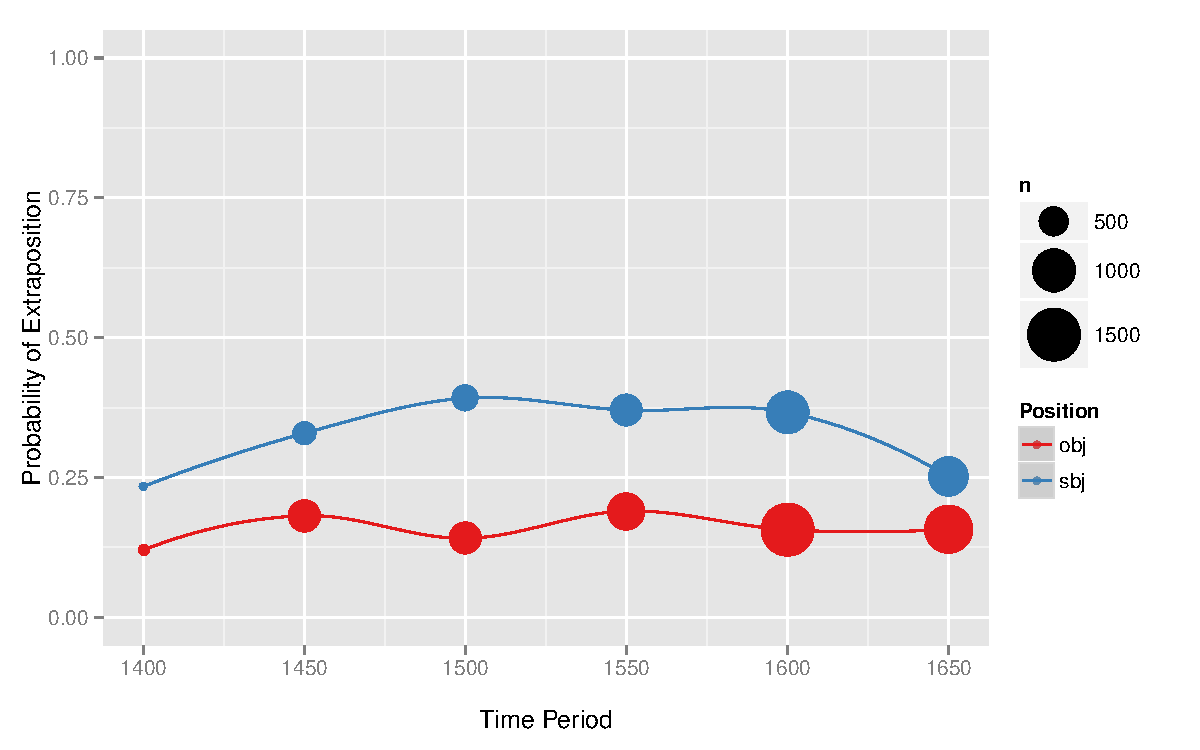
\includegraphics[width=1.1\textwidth]{exSbjObjYearBinned50.pdf}
\end{center}
\end{frame}


 \subsection{Diachronically, Crosslinguistically}

\begin{frame}{Diachronically, Crosslinguistically}
\begin{itemize}

    \item \textbf{Empirical Result:} relative clause extraposition is a change in progress.
        \begin{itemize}
        \item Extraposition is dying, but \textbf{extremely slowly}.
    %    \item It has been mischaracterized as an optional movement.
        \end{itemize}
    \item Same coding query (with minor adaptation) on 7 parsed diachronic corpora (4 language histories).
    \item Both the time-depth and cross-linguistic dimensions were necessary in order to discover the change.
  %  \item Only because we had both dimensions were we able to observe (and confirm) the slowest syntactic change discovered to date.
    \end{itemize}
\end{frame}








\begin{frame}{Diachronically, Crosslinguistically}
\begin{itemize}
	\item \textbf{English:} YCOE \citep{ycoe}, PPCME2 \citep{ppcme2}, PPCEME \citep{ppceme}, PPCMBE \citep{ppcmbe}.
	\item \textbf{Icelandic:} IcePaHC \citep{icepahc09}.
	\item \textbf{Old/Middle French:} MCVF Corpus \\(Martineau, Hirschbühler, Kroch, \& Charles Morin, 2010)\nocite{mcvf}.
	\item \textbf{Historical Portuguese:} Tycho Brahe Corpus of Historical Portuguese \citep{tychobrahe}.
	\end{itemize}
%	\textbf{Hypothesis 1:} the specialization for weight has stabilized, so the effect of weight will be constant over time. \textbf{(Confirmed!)}
%	\textbf{Hypothesis:} the overall rate of relative extraposition will be stable (or without interpretable trend) over time. \textbf{(Rejected!)}

\end{frame}

\begin{frame}{English, over time (N = 18530 clauses)}

\begin{center}
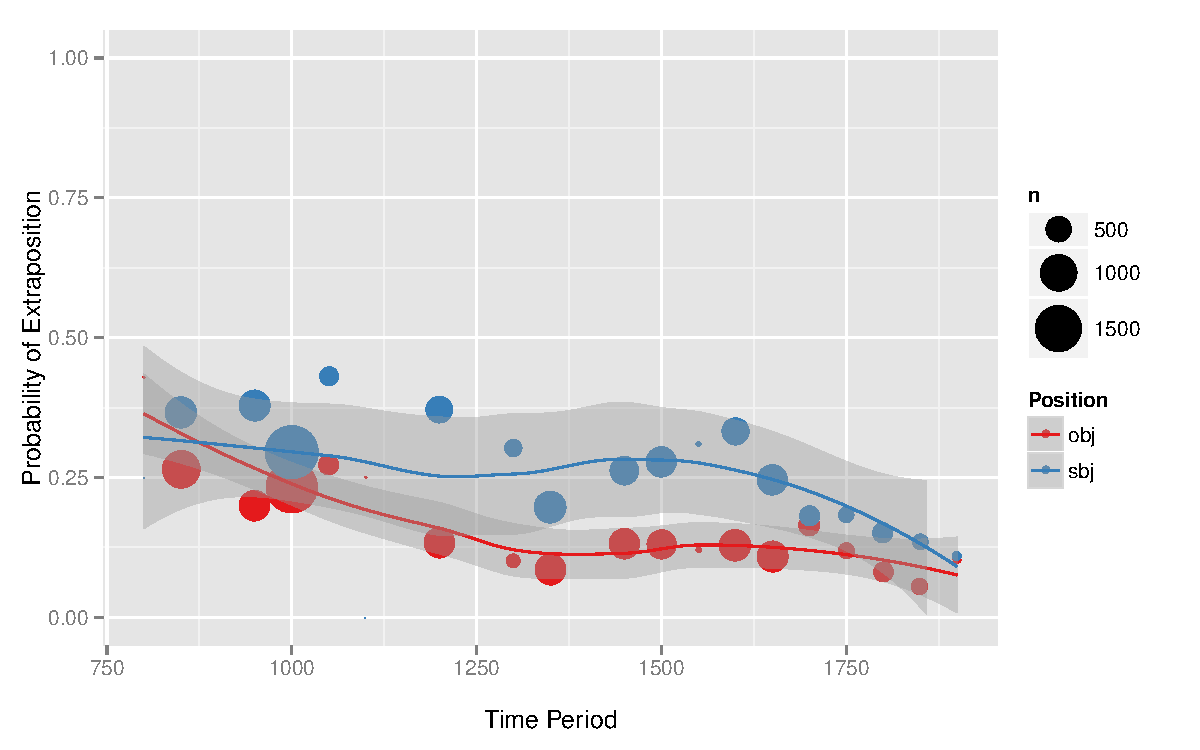
\includegraphics[width=1.1\textwidth]{exSbjObjYearBinned50Loessymeb.pdf}
\end{center}
\end{frame}

\begin{frame}{cf. Yiddish Tense, N = 1030 clauses \\ \small{\citet{wallenberg2013}, building on \citet{santorini1993a}}}

\begin{center}
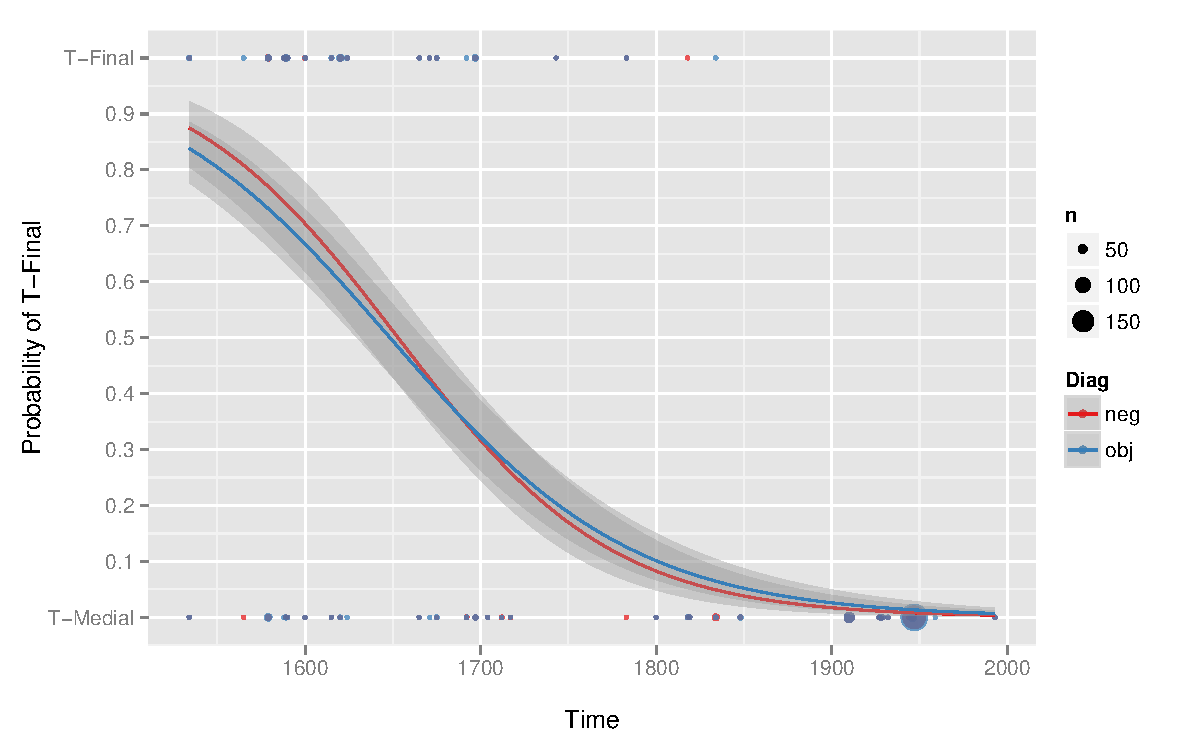
\includegraphics[width=1.05\textwidth]{yiddishLogistic.pdf}
\end{center}
\end{frame}

\begin{frame}{Pause-fillers, \textsl{um} vs. \textsl{uh},  \small{n_{speakers} = 308}\\\small{(\citealt{fruehwald2015}., using \textsl{Philadelphia Neighborhood Corpus})} %n_{tokens} = 25514
%\begin{center}
		}
		
%	\end{center}
		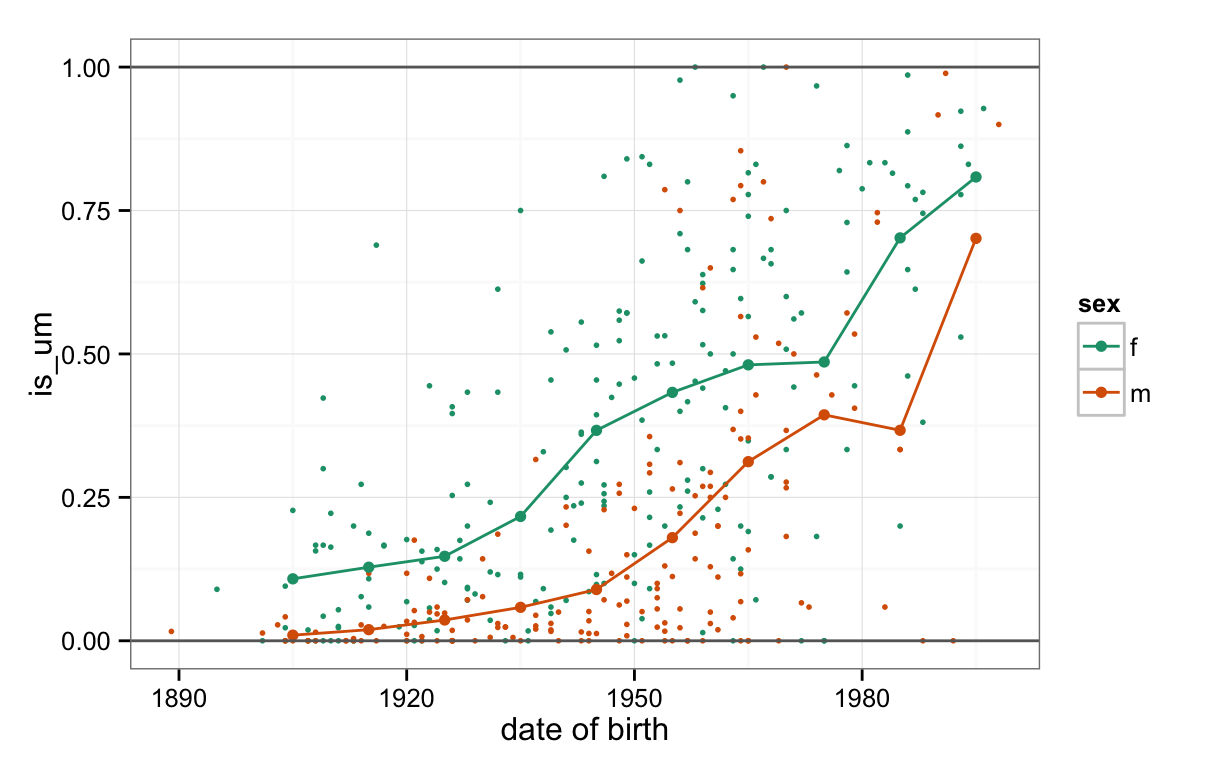
\includegraphics[width=1.16\textwidth]{um.png}
	
	
\end{frame}


\begin{frame}{English, over time (N = 18530 clauses)}

\begin{center}
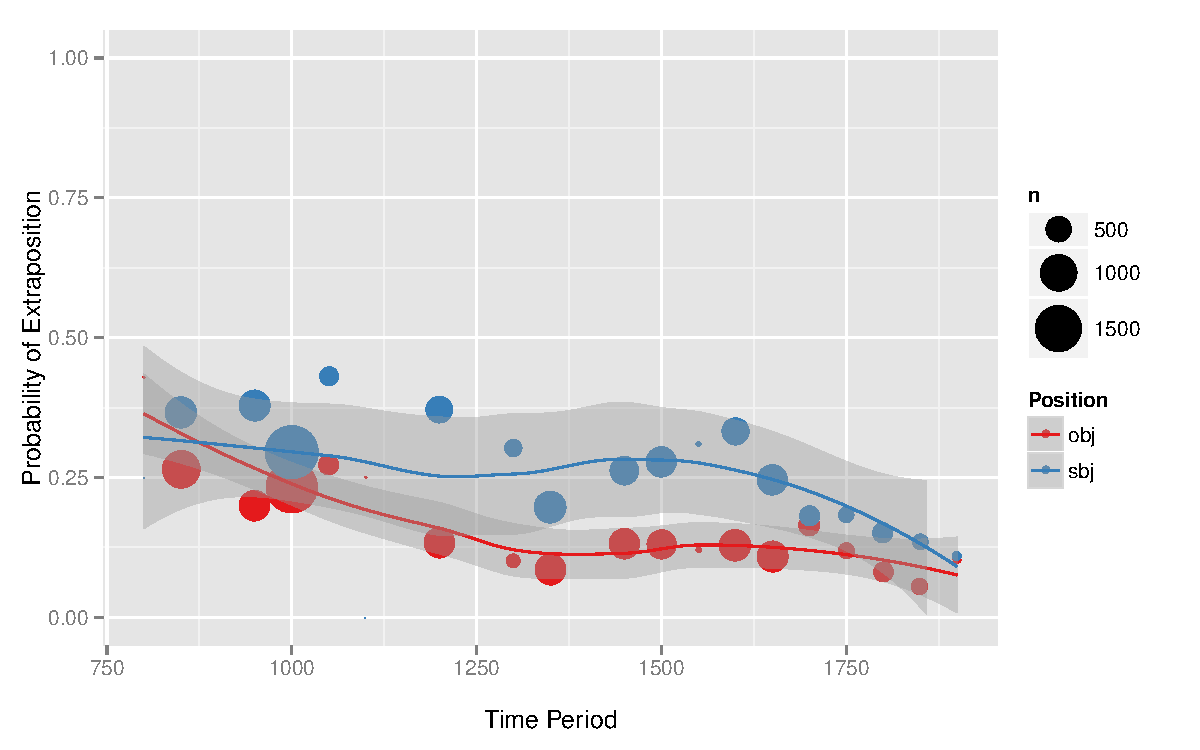
\includegraphics[width=1.1\textwidth]{exSbjObjYearBinned50Loessymeb.pdf}
\end{center}
\end{frame}



\begin{frame}{English, average weight over time (N = 18530)}

\begin{center}
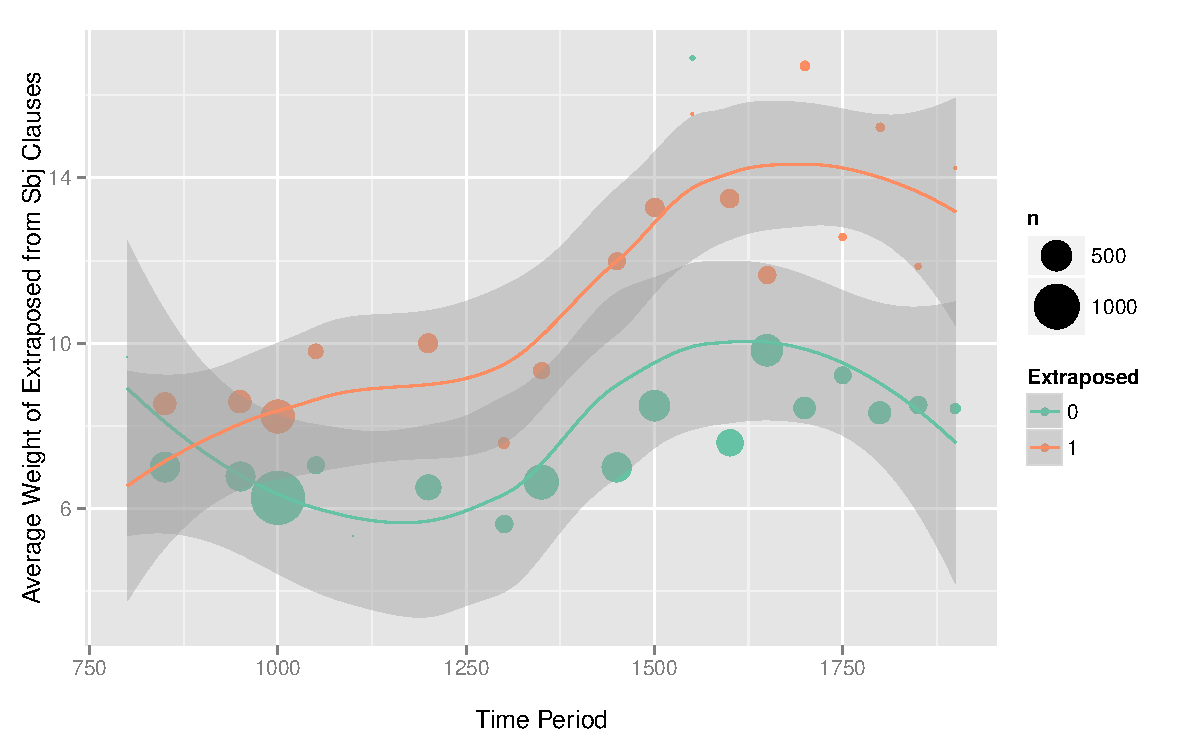
\includegraphics[width=1.1\textwidth]{exWeightYearBinned50Loessymeb.pdf}
\end{center}
\end{frame}

\begin{frame}{Icelandic, over time (N = 3486)}

\begin{center}
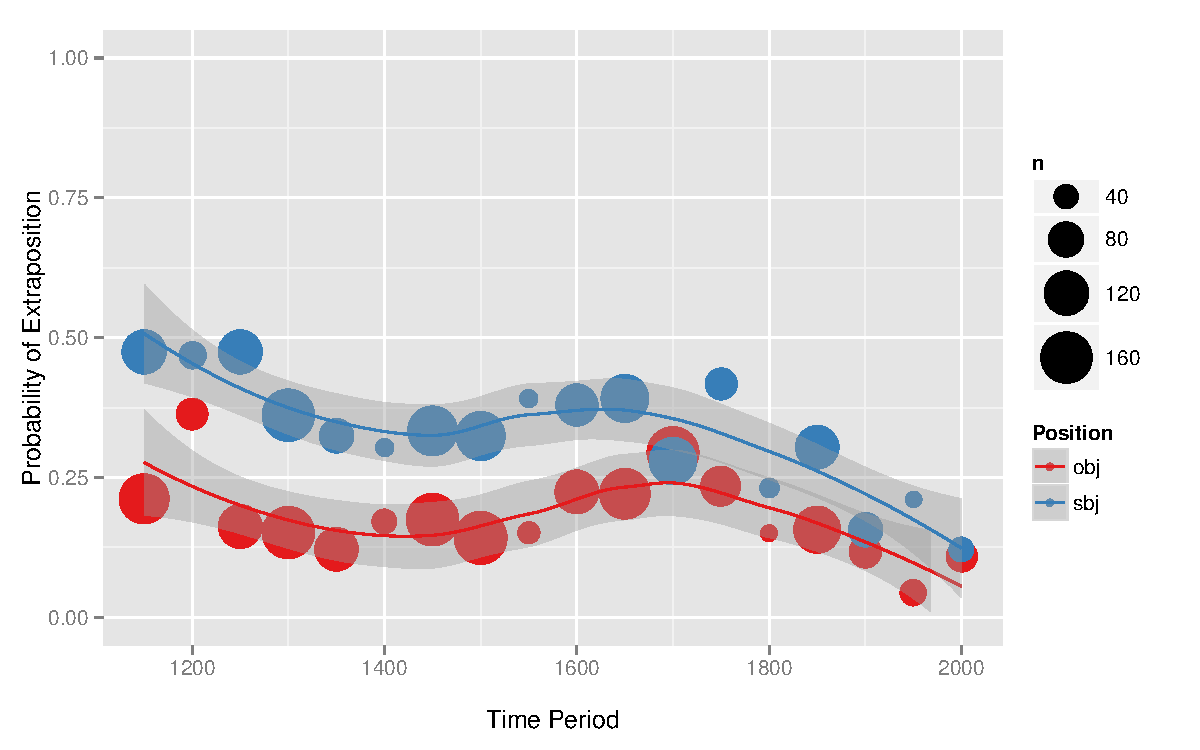
\includegraphics[width=1.1\textwidth]{exSbjObjYearBinned50Loessice.pdf}
\end{center}
\end{frame}


\begin{frame}{Icelandic, average weight over time (N = 3486)}

\begin{center}
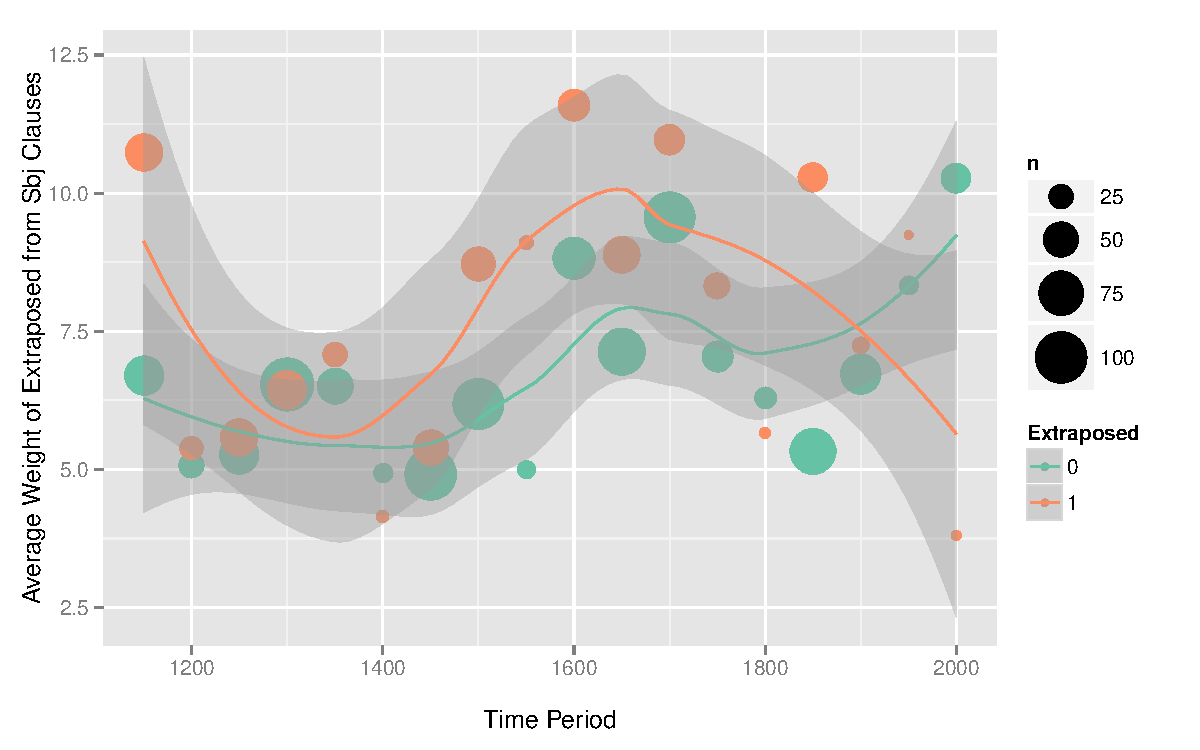
\includegraphics[width=1.1\textwidth]{exWeightYearBinned50Loessice.pdf}
\end{center}
\end{frame}



\begin{frame}{Old/Middle French, over time (N = 8207)}

\begin{center}
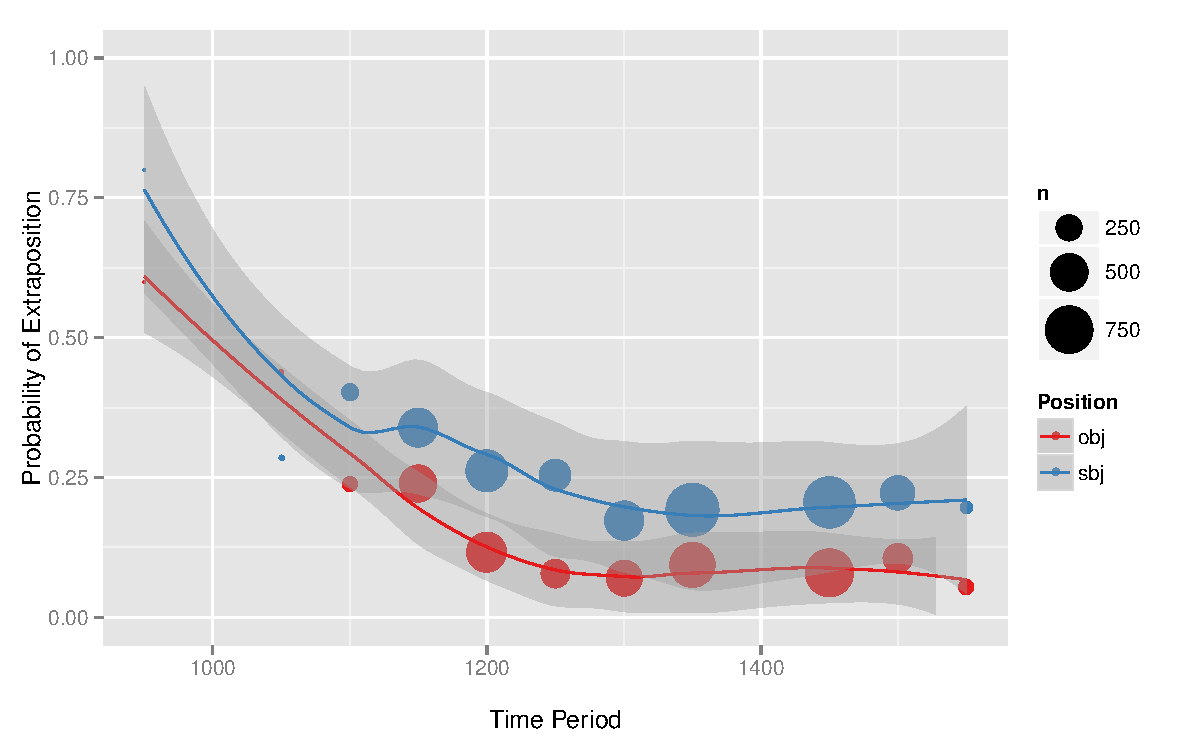
\includegraphics[width=1.1\textwidth]{exSbjObjYearBinned50Loessfre.pdf}
\end{center}
\end{frame}


\begin{frame}{French, average weight over time (N = 8207)}

\begin{center}
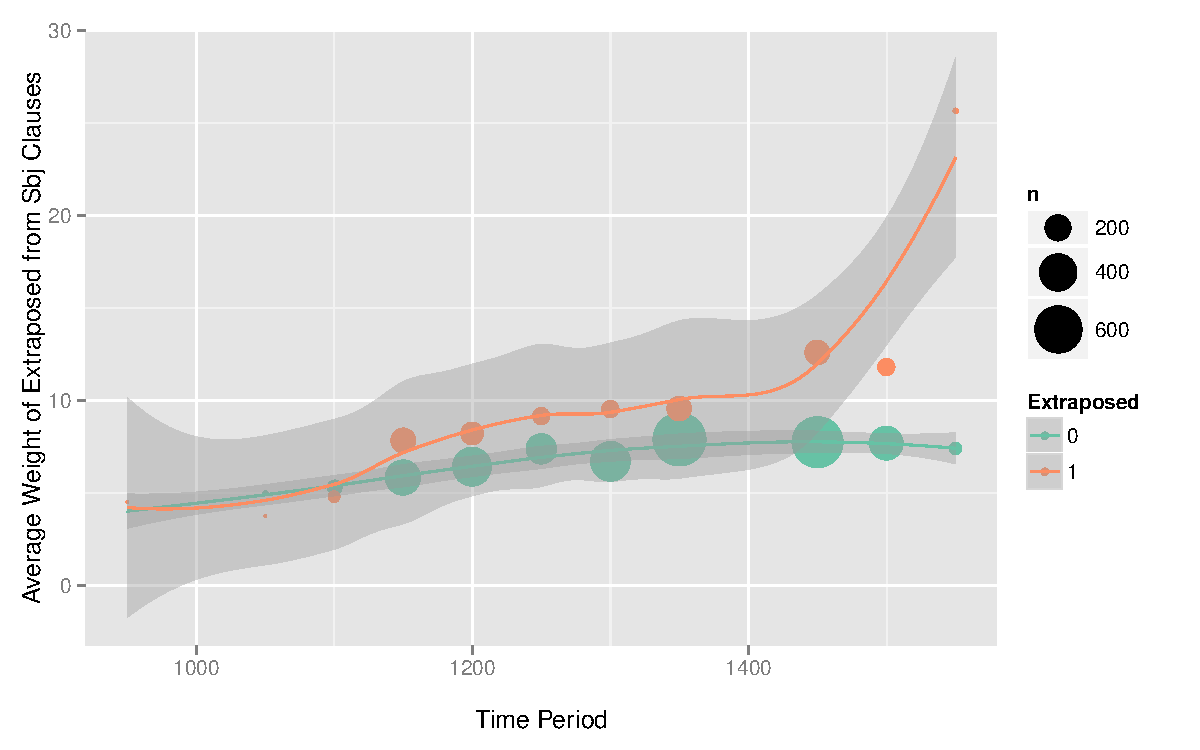
\includegraphics[width=1.1\textwidth]{exWeightYearBinned50Loessfre.pdf}
\end{center}
\end{frame}

\begin{frame}{Portuguese, over time (N = 2398)}

\begin{center}
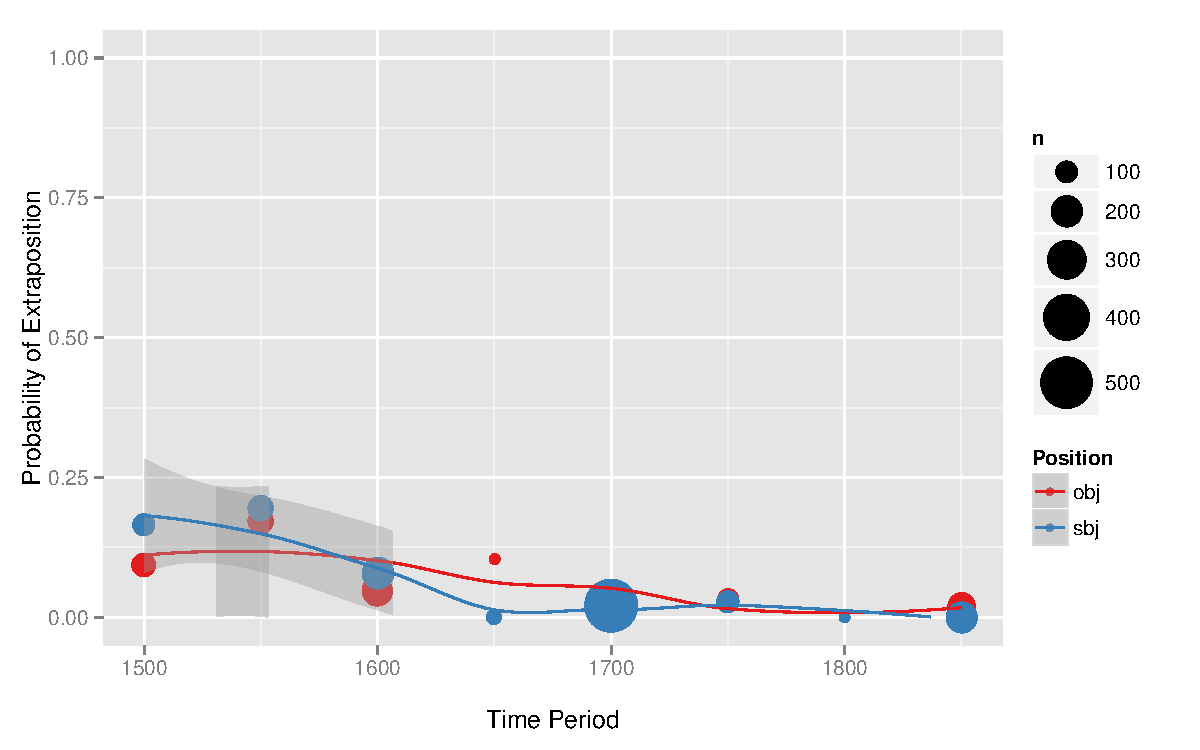
\includegraphics[width=1.1\textwidth]{exSbjObjYearBinned50Loessport.pdf}
\end{center}
\end{frame}


\begin{frame}{Portuguese, average weight over time (N = 2398)}

\begin{center}
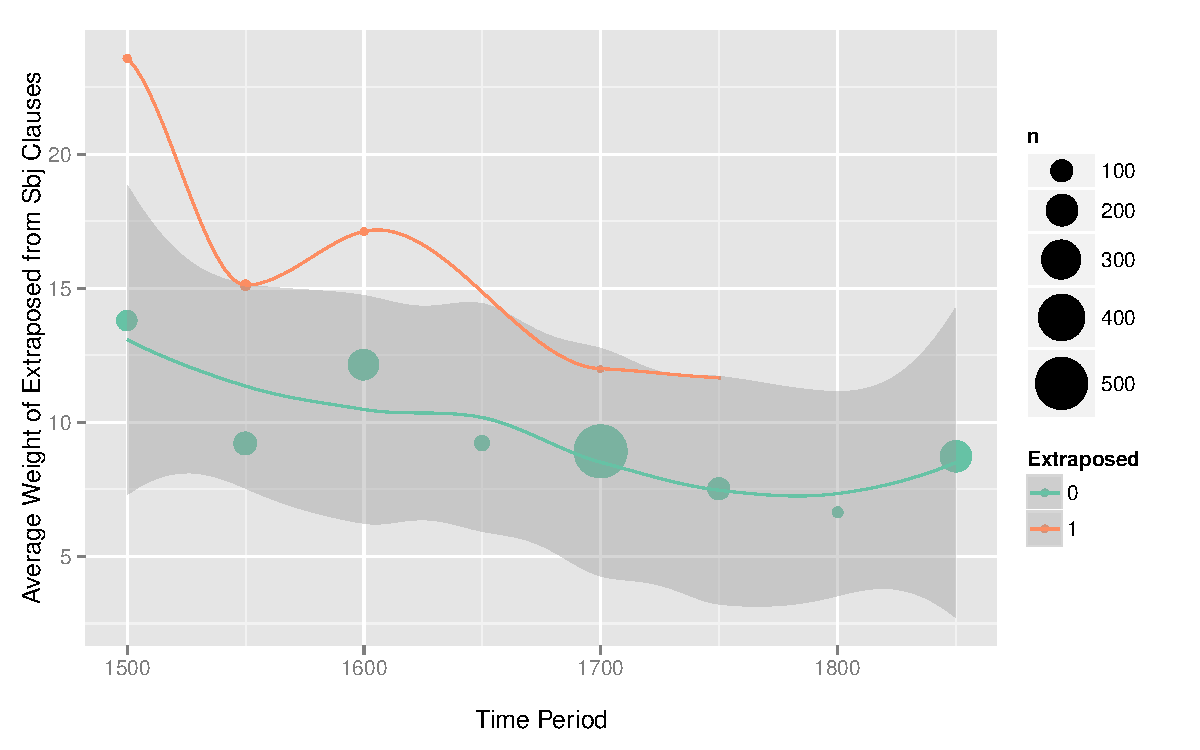
\includegraphics[width=1.1\textwidth]{exWeightYearBinned50Loessport.pdf}
\end{center}
\end{frame}

\begin{frame}{Statistical characteristics of the change}
    \begin{itemize}
    	\item The slope of the decline over time is close to zero for English and Icelandic, but nonzero (p < 10^{-6} for model comparison), and very small (e.g. -10^{-2}) for French and Portuguese (based on logistic regression controlling for weight and other factors). (\textbf{noise} and \textbf{resolution})
	\item Weight has a significant effect in each language, but the effect doesn't change over time.
	\item At least Icelandic and English show the same rate of change (a kind of Constant Rate Effect?), p = 0.47:
\end{itemize}
\end{frame}



\begin{frame}{Four Languages (Subj Ex), over time}

\begin{center}
\includegraphics[width=1.1\textwidth]{exYearBinned50Loessall.pdf}
\end{center}
\end{frame}

\section{Competition}

\begin{frame}{What is in competition?}
    \begin{itemize}
	\item If we take the view of \citet{culicoverrochemont1990}, then relative clauses right-adjoin to various phrasal categories, and extraposition is adjunction to a higher phrasal category.
	\item A principle of interpretation (``Complement Principle'') determines how deeply embedded the interpretation can be.
	\item The doublet, the competing grammars, are actually \textbf{competing adjunction sites with the same interpretation}.
	\end{itemize}
	
\end{frame}

\begin{frame}{The origin of the slow change?}
\begin{exe}
         \ex \label{engcar1} By God's blessing I calculate that the Spirit of Dishonesty shall not get dominion over me; nor the Spirit of Despondency, nor any other evil spirit; \textbf{in which case
all will and must be well}.\\
(Letter by Thomas Carlyle, date: 1835; ID CARLYLE-1835,2,266.176 in PPCMBE)
        \ex \label{engcar3} Nowadays, however, flowers can be arranged in various styles -- some flat, some slightly raised, some bunched boldly in certain
places and forming the piece de resistance of
the whole work -- \textbf{all of which variations depend upon the artistic
perceptions of the operator\textbf}.\\
        (\textsl{Commercial gardening...}, date: 1913;ID WEATHERS-1913,1,9.217 in PPCMBE)
\end{exe}
\end{frame}

\begin{frame}{The origin of the slow change?}
    \begin{exe}

\ex \label{vediccar1} \gll \textbf{yó} \textbf{mártya\d{h}} \textbf{śíś\={i}te} \textbf{áty} \textbf{aktúbhir}, \textbf{m\={\'{a}}} na\d{h} sá ripúr \={i}śata \\
which mortal sharpen-Mid-Sg overly nights-\sc{instr}, not us-\sc{gen} that trickster dominate-Subj3Sg\\
\quad ``As for the mortal who makes himself too sharp by night, may that trickster not gain power over us''\\
\citep[RV 1.36.16, cited in][156]{kiparsky1995}
\end{exe}
\end{frame}



\begin{frame}{Competition? \citet{sauerland2003}}
 \begin{itemize}
	\item Sauerland argues that English relatives are often ambiguous between a \textbf{raising} structure (raising of the ``head'' NP) and an adjoined \textbf{matching} structure, based on binding Principles A and C.
	\item Interestingly, relative clause extraposition seems to be only compatible with the \textbf{matching} structure, the one that does not allow A binding of the ``head'' NP.
\end{itemize}

\begin{exe}
	\ex That picture of John that he likes a lot was just published.
	\ex That picture of himself that John likes a lot was just published.
	\ex ?* That picture of himself was just published that John likes a lot.
\end{exe}
\end{frame}

\begin{frame}{Competition? \citet{sauerland2003}}
 
 Can the loss of extraposition be competition between the matching and raising structures, with matching slowly losing and taking extraposition with it?\\

\end{frame}



\begin{frame}{Competition: matching vs. raising? }

 \begin{itemize}
	\item Can speakers choose the matching structure in order to extrapose? 
		\begin{itemize}
			\item If so, then raising should specialize for in situ, matching for extraposition...why does extraposition decline?
		\end{itemize}
	\item Sauerland claims raising is bad with indefinite NPs, which is where extraposition is most natural, so raising replacing matching would have little effect on extraposition...unless this is part of the slowness, and/or part of the specialization of raising for \textsl{in situ}?
	\item And there's still competing adjunction sites within the matching structure. A 3-way competition?
	\item Is there any evidence to the learner for the matching and raising structures?
\end{itemize}


\end{frame}





\begin{frame}{Summary: Change in Extraposition}

\begin{itemize}

	\item Cross-linguistic Constant Rate Effect: clear for English and Icelandic changes (p = 0.47)
		\begin{itemize} \item Not so clear for Romance, though data is much sparser and the corpora are far less stylistically balanced \end{itemize}
	\item Seeing the change in all the languages makes us more confident that the effect is real in each one.
	\item The change is not at all observable without considerable time-depth.
	\item \textbf{Why the change?} After actuation, extraposition and \textsl{in situ} are competing variants in use, so there can't not be a change, even with partial specialization.
		\begin{itemize}
		\item Specialization can only be partial along the (continuous) weight dimension.
		%\item Perhaps a small selectional advantage has asserted itself in the usage-overlap, but can only do so slowly because the overlap is limited.
		\end{itemize}
\item Perhaps \citet{kiparsky1995} identifies a change that goes beyond Proto-Germanic, though hard to test.
%	\item The questions we can ask are now far more nuanced, given cross-linguistic and extended diachronic dimensions.
\end{itemize}

\end{frame}


\begin{frame}{More Nuanced Questions}
\begin{itemize}
	\item Any role for Sauerland's competing relative clause structures? How would we observe them diachronically?
	\item Relative clause extraposition is restricted in its syntactic context in modern Portuguese \citep{cardoso2011, cardoso2012}; specialization? cause and effect?
	\item How likely is a change like this to result from fixation by drift in a finite population (of utterances) and speakers through random death? (\citealt{moran1958}; see \citealt{nowak2006} for an overview and references).
%	\item \textbf{Note:} topicalization in English has slowly declined from 1750 through the 20th c. (A. Kroch, p.c.).
\end{itemize}
\end{frame}


\section{Specialization}
\begin{frame}{Specialization in Acquisition: active or passive?}
		\begin{enumerate}
			\item Identify a domain of specialization:
				\begin{itemize}
					\item \textbf{Actively}, creatively, by the child innovating \textsl{de novo}?
					\item \textbf{Passively}, though random sampling of finite populations of utterances?
				\end{itemize}
			\item For categorical variants along categorical dimensions, uncouple tracked frequencies of variants.
			\item Specialization completes in a categorical dimension:
			\begin{itemize}
				\item \textbf{Actively}, by punishing one variant when the other is rewarded?
				\item \textbf{Passively}, by allowing whatever evolutionary dynamics hold in the different contexts play out, whether the outcome is different or not?
			\end{itemize}
		\end{enumerate}
\end{frame}

\begin{frame}{Specialization in Acquisition: active or passive?}
		\begin{enumerate}
			\item For categorical variants along continuous dimensions, uncouple tracked means of variants in the dimension of specialization.
			\item Specialization completes in a continuous dimension:
			\begin{itemize}
				\item \textbf{Actively}, by moving the means of variants away from each other?
				\item \textbf{Passively}, by allowing the means to potentially move away from each other?
			\end{itemize}
		\end{enumerate}
\end{frame}


\begin{frame}{Specialization in Acquisition as a Challenge for Bad Data}
		\begin{itemize}
			\item This model of specialization is an extension of \citet{yang2000, yang2002}.
			\item Can we observe specialization, and the choosing of domains of specialization diachronically?
			\item Can we observe it in acquisition?
				\begin{itemize}
					\item Production data may not be good enough here.
				\end{itemize}
			\item Can we observe either well enough to test active vs. passive hypotheses?
		\end{itemize}
\end{frame}

\section{Conclusion}

\begin{frame}{Conclusion: embedding and transition}
		\begin{itemize}
			\item Relative clause extraposition is in decline, and we can just about link it to:
			\begin{itemize}
			\item a larger theory of syntactic representations \\(\textbf{grammatical embedding})
			\item a theory of language specialization in acquisition (\textbf{extragrammatical embedding}).
			\end{itemize}
			\item There is a level of syntactic detail that is currently beyond our/my ability to test (?).
			\item There is a level of detail in the theory of specialization that is currently beyond our/my ability to test (?).
			\item The information on \textbf{transition} is based on very high-quality, expensive data (parsed diachronic corpora, beyond the ability of an individual to produce).%which allows us to observe a lot more than we could before.
			\item It is still noisy, and we would like finer resolution as we tackle questions above, and e.g. selection vs. drift.
		\end{itemize}
\end{frame}


\begin{frame}{Acknowledgements}
\begin{center}
Thank you first to Josef Fruehwald for working out many of these ideas with me, and to Anthony Kroch and Betsy Sneller for much discussion of these issues. Thanks to Anton Karl Ingason for use of his CS queries. Also Aaron Ecay, Ricardo Bermúdez-Otero, Caitlin Light, Laurel Mackenzie, George Walkden, and anonymous reviewers.
\vspace{5mm}\\
Extraposition Study: \texttt{github.com/joelcw/tyneside/tree/master/extraposition}
\end{center}
\end{frame}


\begin{frame}[allowframebreaks]
\frametitle{References}
\newcommand*{\newblock}{natbib}
\bibliographystyle{linquiry2}
\bibliography{joelrefs}
\end{frame}

\end{document}